\documentclass[aspectratio=169]{beamer}
\usetheme{default}
\usefonttheme{professionalfonts}
\renewcommand{\familydefault}{\sfdefault}
\usepackage[T1]{fontenc}
\usepackage{helvet}
\usepackage{booktabs}
\usepackage{tikz}
\usepackage{xcolor}

\definecolor{imsbblue}{RGB}{31,95,140}
\definecolor{imsbdark}{RGB}{20,63,93}
\definecolor{imsbgrey}{RGB}{90,90,90}

\setbeamercolor{structure}{fg=imsbblue}
\setbeamercolor{frametitle}{bg=imsbblue,fg=white}
\setbeamercolor{title}{fg=imsbdark}
\setbeamercolor{caption name}{fg=imsbblue}
\setbeamercolor{itemize item}{fg=imsbblue}
\setbeamercolor{itemize subitem}{fg=imsbblue}

\setbeamertemplate{navigation symbols}{}
\setbeamertemplate{itemize item}{\small\raise0.3pt\hbox{\textbullet}}
\setbeamertemplate{itemize subitem}{\scriptsize\raise0.3pt\hbox{--}}

\setbeamertemplate{frametitle}{%
  \nointerlineskip
  \begin{beamercolorbox}[wd=\paperwidth,ht=2.6ex,dp=1.2ex,leftskip=0.3cm,rightskip=0.3cm]{frametitle}%
    \usebeamerfont{frametitle}\insertframetitle%
  \end{beamercolorbox}%
}

\setbeamertemplate{footline}{%
  \leavevmode%
  \hbox{%
  \begin{beamercolorbox}[wd=.34\paperwidth,ht=2.4ex,dp=1ex,center]{author in head/foot}%
    \usebeamercolor[fg]{}\tiny\insertshortauthor%
  \end{beamercolorbox}%
  \begin{beamercolorbox}[wd=.4\paperwidth,ht=2.4ex,dp=1ex,center]{title in head/foot}%
    \tiny\insertshorttitle%
  \end{beamercolorbox}%
  \begin{beamercolorbox}[wd=.26\paperwidth,ht=2.4ex,dp=1ex,center]{date in head/foot}%
    \tiny\insertshortdate{}\hspace*{1em}\insertframenumber/\inserttotalframenumber%
  \end{beamercolorbox}}%
  \vskip0pt%
}
\setbeamercolor{author in head/foot}{bg=imsbdark,fg=white}
\setbeamercolor{title in head/foot}{bg=imsbdark,fg=white}
\setbeamercolor{date in head/foot}{bg=imsbdark,fg=white}

\setbeamertemplate{title page}{%
  \vskip2.0em
  {\usebeamercolor[fg]{title}\Large\bfseries\inserttitle\par}
  \vskip1.2em
  {\large\insertauthor\par}
  \vskip0.4em
  {\color{black}\insertinstitute\par}
  \vskip1.4em
  {\insertdate\par}
}

\usetikzlibrary{arrows.meta,positioning,shapes.geometric,fit,backgrounds,calc}
\tikzset{
  box/.style={draw=imsbblue,thick,rounded corners,align=center,fill=imsbblue!7,inner sep=5pt,font=\footnotesize},
  alt/.style={draw=imsbgrey,thick,rounded corners,align=center,fill=imsbgrey!10,inner sep=5pt,font=\footnotesize},
  lab/.style={align=center,font=\scriptsize,text=black},
  arr/.style={-{Stealth[length=2.4mm]},thick,draw=imsbdark},
  line/.style={thick,draw=imsbblue},
}
\newcommand{\refline}[1]{\vfill{\scriptsize\color{black} #1}}
\newcommand{\figslot}[2]{%
  \begin{center}
  \setlength{\fboxsep}{9pt}%
  \fcolorbox{imsbblue}{imsbblue!4}{\parbox{0.84\linewidth}{\centering\footnotesize
  \textcolor{imsbblue}{\textbf{[ figure slot ]}}\\[3pt] #1 \\[4pt]
  {\scriptsize\color{black} suggested source: #2}}}
  \end{center}}
\usepackage{listings}
\usepackage{xcolor}
\usepackage{url}
\usepackage{hyperref}

\lstset{
  basicstyle=\ttfamily\scriptsize,
  keywordstyle=\color{imsbblue}\bfseries,
  commentstyle=\color{black}\itshape,
  stringstyle=\color{imsbdark},
  showstringspaces=false,
  columns=fullflexible,
  breaklines=true,
  frame=single,
  rulecolor=\color{imsbblue!40},
  language=Python,
}

\title{Topology-aware learning for higher-order cell-cell interaction in spatial transcriptomics:\\Introduction to spatial transcriptomics}
\author{Lucia Testa, Robin Khatri}
\institute{Institute of Medical Systems Bioinformatics, UKE}
\date{LOGML summer school}

\begin{document}

\begin{frame}[plain]\titlepage\end{frame}

\begin{frame}{This module}
  Bringing a machine-learning and mathematics background to a live problem in spatial
  biology.
  \vskip0.5em
  \begin{itemize}
    \item \textbf{Part 1 (this talk).} What spatial transcriptomics is, the data, the
      libraries, the standard methods, and where they break.
    \item \textbf{Part 2 (labs).} Two notebooks: an introduction to the data, libraries and
      workflow, then spatial methods and the open challenges.
    \item \textbf{Part 3.} The higher-order / topological project (next part).
  \end{itemize}
  \vskip0.3em
  \refline{Repo: \url{https://github.com/robinredX/st-topo-aware-learning-logml}}
\end{frame}

% ---------------------------------------------------------------------------
\section{Spatial transcriptomics}

\begin{frame}{Why spatial?}
  \begin{columns}[T]
  \begin{column}{0.54\textwidth}
  Dissociation-based scRNA-seq tells you \emph{which} cells are present but throws away
  \emph{where} they were.
  \vskip0.5em
  Tissue function lives in \textbf{organisation}: who sits next to whom, tissue
  compartments, local signalling hubs. Spatial transcriptomics (ST) keeps the coordinates,
  so we can ask those questions directly.
  \vskip0.5em
  For an ML audience: ST hands you a \textbf{geometry} (points in a plane) with a
  high-dimensional signal (expression) attached, plus rich structure to exploit.
  \end{column}
  \begin{column}{0.44\textwidth}
  \centering
  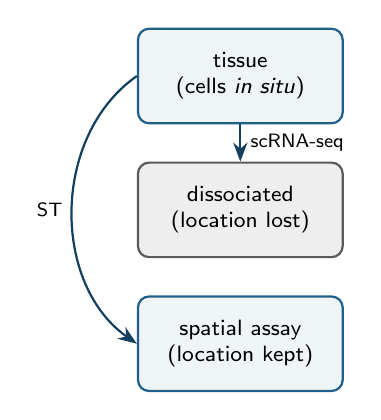
\begin{tikzpicture}[scale=0.85]
    \node[box,minimum width=2.6cm,minimum height=1.2cm] (t) at (0,2) {tissue\\(cells \textit{in situ})};
    \node[alt,minimum width=2.6cm,minimum height=1.2cm] (d) at (0,0) {dissociated\\(location lost)};
    \node[box,minimum width=2.6cm,minimum height=1.2cm] (s) at (0,-2) {spatial assay\\(location kept)};
    \draw[arr] (t) -- node[lab,right]{scRNA-seq} (d);
    \draw[arr] (t.west) to[bend right=55] node[lab,left]{ST} (s.west);
  \end{tikzpicture}
  \end{column}
  \end{columns}
\end{frame}

\begin{frame}{Two families of technology}
  \begin{columns}[T]
  \begin{column}{0.49\textwidth}
  \textbf{Spot / capture based} (Visium, Slide-seq, HD)
  \begin{itemize}
    \item barcoded spots on a slide; \emph{whole transcriptome}
    \item a spot mixes several cells (Visium $\sim$1--10); needs deconvolution
    \item coarse spatial resolution
  \end{itemize}
  \end{column}
  \begin{column}{0.49\textwidth}
  \textbf{Imaging / probe based} (Xenium, MERFISH, CosMx)
  \begin{itemize}
    \item image individual transcripts; \emph{single-cell, subcellular}
    \item a fixed gene \textbf{panel} ($\sim$100--500 genes)
    \item needs cell \textbf{segmentation}
  \end{itemize}
  \end{column}
  \end{columns}
  \vskip0.6em
  \begin{center}\footnotesize
  The trade-off: \textbf{transcriptome-wide but low resolution} vs \textbf{single-cell but
  targeted}. This module uses \textbf{Xenium} (single-cell, so cells are real nodes).
  \end{center}
  \refline{Marx. Method of the Year 2020. \emph{Nat Methods} 2021; Moses \& Pachter. Museum of spatial transcriptomics. \emph{Nat Methods} 2022.}
\end{frame}

\begin{frame}{The data object}
  \begin{columns}[T]
  \begin{column}{0.56\textwidth}
  Everything is an \textbf{AnnData}: a cell $\times$ gene matrix plus annotations.
  \begin{itemize}
    \item \texttt{adata.X} -- expression (cells $\times$ genes)
    \item \texttt{adata.obs} -- per-cell table (cell type, sample, QC)
    \item \texttt{adata.obsm['spatial']} -- $x,y$ coordinates
    \item \texttt{adata.obsp[...]} -- the \textbf{spatial graph}
  \end{itemize}
  \vskip0.4em
  The spatial graph (Delaunay / kNN / radius) turns coordinates into a discrete structure
  every downstream method builds on.
  \end{column}
  \begin{column}{0.42\textwidth}
  \centering
  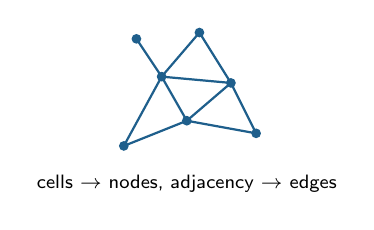
\begin{tikzpicture}[scale=0.8]
    \foreach \x/\y in {0/0,1/0.4,0.6/1.1,1.7/1.0,1.2/1.8,0.2/1.7,2.1/0.2}{\fill[imsbblue] (\x,\y) circle (2.2pt);}
    \draw[line] (0,0)--(1,0.4)--(0.6,1.1)--(0,0);
    \draw[line] (1,0.4)--(1.7,1.0)--(0.6,1.1);
    \draw[line] (1.7,1.0)--(1.2,1.8)--(0.6,1.1);
    \draw[line] (0.6,1.1)--(0.2,1.7); \draw[line] (1,0.4)--(2.1,0.2)--(1.7,1.0);
    \node[lab] at (1,-0.6) {cells $\to$ nodes, adjacency $\to$ edges};
  \end{tikzpicture}
  \end{column}
  \end{columns}
\end{frame}

\begin{frame}{The libraries}
  \begin{itemize}
    \item \textbf{scanpy / anndata} -- the single-cell backbone (IO, QC, normalisation,
      clustering, embeddings).
    \item \textbf{squidpy} -- spatial extension: neighbour graphs, neighbourhood enrichment,
      co-occurrence, Ripley, \texttt{ligrec} for communication.
    \item \textbf{spatialdata / spatialdata-io} -- readers and a coordinate-aware container
      for Xenium/Visium (images, shapes, points).
    \item \textbf{torch + torch-geometric} -- graph neural nets on the spatial graph.
    \item \textbf{gudhi / toponetx / topomodelx} -- topology: simplicial complexes,
      persistence, and higher-order message passing (Part 2).
    \item \textbf{liana / decoupler} -- ligand-receptor resources and consensus CCC.
  \end{itemize}
  \refline{Wolf et al. Scanpy. \emph{Genome Biol} 2018; Palla et al. Squidpy. \emph{Nat Methods} 2022.}
\end{frame}

% ---------------------------------------------------------------------------
\section{Methods and challenges}

\begin{frame}{The core tasks}
  \centering
  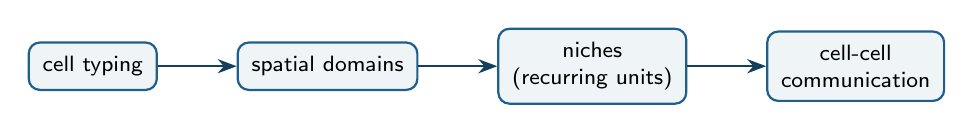
\begin{tikzpicture}[node distance=6mm and 10mm]
    \node[box] (a) {cell typing};
    \node[box,right=of a] (b) {spatial domains};
    \node[box,right=of b] (c) {niches\\(recurring units)};
    \node[box,right=of c] (d) {cell-cell\\communication};
    \draw[arr] (a)--(b); \draw[arr] (b)--(c); \draw[arr] (c)--(d);
  \end{tikzpicture}
  \vskip0.8em
  \begin{itemize}
    \item \textbf{Spatial domains}: partition the tissue into coherent regions from
      expression \emph{and} position.
    \item \textbf{Niches}: recurring multi-cell neighbourhoods (the composition is the label).
    \item \textbf{Communication}: which cell types signal to which, and where.
  \end{itemize}
  These are the tasks a topology-aware model can target.
\end{frame}

\begin{frame}{Spatial domains: the method landscape}
  Almost all are \textbf{graph} methods, expression smoothed or attended over the spatial
  graph:
  \begin{itemize}
    \item \textbf{SpaGCN} -- graph convolution over spots + histology.
    \item \textbf{STAGATE} -- graph attention autoencoder.
    \item \textbf{BANKSY} -- augment each cell with its neighbourhood mean and azimuthal
      gradient, then cluster (fast, strong baseline).
    \item \textbf{CellCharter / nichePCA} -- cluster neighbourhood-aware embeddings into niches.
  \end{itemize}
  \vskip0.4em
  \textbf{Common thread:} a node feature plus message passing on the spatial graph, the graph
  falls out naturally from the coordinates.
  \refline{Hu et al. SpaGCN. \emph{Nat Methods} 2021; Dong \& Zhang. STAGATE. \emph{Nat Commun} 2022; Singhal et al. BANKSY. \emph{Nat Genet} 2024; Varrone et al. CellCharter. \emph{Nat Genet} 2024.}
\end{frame}

\begin{frame}{Cell-cell communication: the standard logic}
  \begin{columns}[T]
  \begin{column}{0.56\textwidth}
  Score a \textbf{ligand-receptor (LR)} pair: ligand $L$ high in cell type $A$, receptor
  $R$ high in a neighbouring type $B$.
  \begin{itemize}
    \item \textbf{Non-spatial:} CellPhoneDB, CellChat, NicheNet; LIANA unifies them.
    \item \textbf{Spatial-aware:} squidpy \texttt{ligrec}, stLearn, COMMOT (optimal
      transport), NCEM.
  \end{itemize}
  \vskip0.3em
  The score lives on an \textbf{edge} $A\!-\!B$. It is \textbf{pairwise by construction}.
  \end{column}
  \begin{column}{0.42\textwidth}
  \centering
  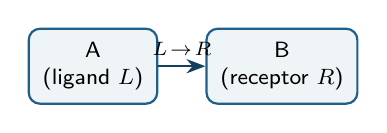
\begin{tikzpicture}[scale=1]
    \node[box] (A) at (0,0) {A\\(ligand $L$)};
    \node[box] (B) at (2.4,0) {B\\(receptor $R$)};
    \draw[arr] (A)--node[lab,above]{$L\!\to\!R$}(B);
  \end{tikzpicture}
  \end{column}
  \end{columns}
  \refline{Efremova et al. CellPhoneDB. \emph{Nat Protoc} 2020; Jin et al. CellChat. \emph{Nat Commun} 2021; Dimitrov et al. LIANA. \emph{Nat Commun} 2022; Cang \& Nie. COMMOT. \emph{Nat Methods} 2023.}
\end{frame}

\begin{frame}{Challenges (where you come in)}
  \begin{itemize}
    \item \textbf{Segmentation.} Cell boundaries are estimated; mis-assigned transcripts
      corrupt co-expression and communication.
    \item \textbf{Sparsity and noise.} Few counts per cell/gene; targeted panels miss genes.
    \item \textbf{Scale.} Millions of cells per slide; methods must be graph-sparse and
      batched.
    \item \textbf{Batch / patient effects} across samples and conditions.
    \item \textbf{Beyond pairwise.} Graphs and LR edges capture pairwise relations; relays
      and multi-cell niches are higher order, the focus of the project (next part).
  \end{itemize}
\end{frame}

% ---------------------------------------------------------------------------
\section{Higher-order interactions}

\begin{frame}{Where this module goes: beyond pairwise}
  The pairwise picture misses interactions that are intrinsically \textbf{higher order}:
  \begin{itemize}
    \item \textbf{Relay signalling.} $A\!\to\!B\!\to\!C$: the meaningful unit is the chain,
      which a pairwise scan splits into two unrelated hits.
    \item \textbf{Multi-cell niches.} A glomerular crescent or an immune focus is a
      coordinated group of three or more cell types, not a single edge.
  \end{itemize}
  \vskip0.3em
  \begin{center}\footnotesize
  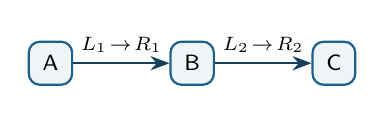
\begin{tikzpicture}[scale=1]
    \node[box] (A) at (0,0) {A};
    \node[box] (B) at (1.8,0) {B};
    \node[box] (C) at (3.6,0) {C};
    \draw[arr] (A)--node[lab,above]{$L_1\!\to\!R_1$}(B);
    \draw[arr] (B)--node[lab,above]{$L_2\!\to\!R_2$}(C);
  \end{tikzpicture}
  \end{center}
  \vskip0.2em
  This is the project's focus: \textbf{CellNEST} (attention-based relay networks) and
  \textbf{topological deep learning} (message passing over triangles and higher cells).
  \textbf{Lucia covers both in detail next}.
\end{frame}

% ---------------------------------------------------------------------------
\section{The project}

\begin{frame}{The dataset}
  \textbf{Human kidney Xenium} (GSE294965): ANCA vasculitis, lupus nephritis, anti-GBM and
  control biopsies; $\sim$3.2M cells, single-cell resolution.
  \begin{itemize}
    \item One AnnData (\texttt{GSE294965\_processed\_data.h5ad}, $\sim$3.9 GB). Download once,
      point \texttt{ST\_DATA} at it (see \texttt{data/datasets.md}).
    \item Disease context makes higher-order structure biologically real: crescents,
      immune infiltrates, injured tubules are multi-cell units.
    \item Prefer a smaller tissue? Any 10x Xenium public dataset works
      (\url{10xgenomics.com/datasets}). The notebooks only need coordinates + a cell-type
      label.
  \end{itemize}
  \refline{Ligand-receptor resources ship in \texttt{data/}: a gene-symbol LR table + the canonical CellPhoneDB.}
\end{frame}

\begin{frame}{The notebooks}
  \begin{itemize}
    \item \textbf{01 -- introduction.} Load a Xenium section, the AnnData object, QC,
      normalisation, cell types, spatial visualisation.
    \item \textbf{02 -- spatial methods and challenges.} Neighbourhood graph, neighbourhood
      enrichment, domains (nichePCA), a brief \texttt{ligrec}, and the open challenges.
  \end{itemize}
  \vskip0.3em
  The higher-order / topological project builds on this in the next part. \texttt{src/topo\_utils.py}
  ships the shared helpers (spatial graph, graph-to-complex lift) for it.
\end{frame}

\begin{frame}{Project directions}
  \begin{itemize}
    \item \textbf{Higher-order CCC.} Lift LR scoring to triangles; do high-scoring motifs
      localise to known niches (crescents, immune foci)?
    \item \textbf{Topology vs graph.} Same section, same task (domain segmentation): GCN/GAT
      baseline vs a TopoModelX simplicial model. Where does higher order help?
    \item \textbf{Denoising / reconstruction.} Mask genes or cells; does higher-order
      propagation recover signal better than pairwise?
    \item \textbf{Benchmark the inductive bias.} When is the extra machinery worth it?
  \end{itemize}
\end{frame}

\begin{frame}{References}
  \scriptsize
  \begin{itemize}
    \item Marx. Method of the Year 2020: spatially resolved transcriptomics. \emph{Nat Methods} 2021;
      Moses \& Pachter. Museum of spatial transcriptomics. \emph{Nat Methods} 2022.
    \item Palla et al. Squidpy. \emph{Nat Methods} 2022; Wolf et al. Scanpy. \emph{Genome Biol} 2018.
    \item Hu et al. SpaGCN 2021; Dong \& Zhang. STAGATE 2022; Singhal et al. BANKSY 2024;
      Varrone et al. CellCharter 2024.
    \item Efremova et al. CellPhoneDB. \emph{Nat Protoc} 2020; Jin et al. CellChat 2021;
      Dimitrov et al. LIANA. \emph{Nat Commun} 2022; Cang \& Nie. COMMOT. \emph{Nat Methods} 2023.
    \item Fatema et al. CellNEST. \emph{Nat Methods} 2025.
    \item Bodnar et al. WL go cellular / topological. \emph{ICML/NeurIPS} 2021;
      Papillon et al. TopoModelX / TopoNetX 2023; Hajij et al. Topological deep learning 2023.
  \end{itemize}
\end{frame}

\end{document}
